\documentclass[12pt]{article}

% PACKAGES

\usepackage{amsmath}
\usepackage{fancyvrb}
\usepackage{hyperref}
\usepackage{multicol}
\usepackage{wrapfig}
\usepackage{graphicx}
\graphicspath{ {./images/} }

% CUSTOM COMMANDS

\newcommand{\row}[1]{\texttt{#1}}
\newcommand{\br}[0]{\vspace{10pt} \noindent}
\newcommand{\footurl}[1]{\footnote{\url{#1}}}
\newcommand{\nth}[2]{#1\textsuperscript{#2}}

% TITLE

\title{Insert Report Title Here}
\author{Benjamin White-Horne \\ \emph{Oxford University}}



\begin{document}

\maketitle



\pagebreak

\section*{Abstract}

This project concerns the designing and prototyping of Jigsaw, an application to help change ringing
composers to compose while requiring as little change to their workflow as possible.  In other
words, Jigsaw aims to be to composers is to Microsoft Word is to writers.  Additionally, I hope that
the addition of a beginner-friendly visual tool will make composing easier for people to get into
(MU/DA:\@ please reword this --- thanks).  Jigsaw is currently deployed as a static web app using
GitHub pages.

Whilst writing Jigsaw I also created BellFrame, a fast and idiomatic Rust library which provides
easy-to-use datatypes for ubiquitous concepts in change ringing.  BellFrame has good documentation
with code examples, and is in itself a very useful asset.  Once its API is more stable, I will
publish it to Rust's package repository for general use.

\br{}Change ringing is an art form which is almost exclusive to England, where people ring sets of
bells in continually evolving sequences, known as `changes' or `rows'.  The art of `composing'
concerns designing sequences of rows for ringers to perform, and predates computers by several
centuries (the earliest surviving record of composing come from Fabian Stedman in the 1700s).

Compositions are at their core sequences of permutations and are therefore extremely amenable to
both mathematical and computer analysis.  Some parts of composition have already been well
automated, including brute-force generation of compositions, but there are very few user-friendly
tools for composers.  By prototyping Jigsaw, I have explored one possible way to fill this gap.



\pagebreak

\tableofcontents



\pagebreak

\section{Introduction}

\subsection{Change Ringing and Composing}

\subsection{Project Goals}\label{sec:design-goals}

This project concerns prototyping an application to \emph{aid} composers whilst requiring the
smallest possible change to their existing workflow.  This is analogous to what Microsoft Word
provides for writers --- a kind of `automated paper' which automatically annotates your work with
data that is tedious to compute manually whilst still providing it in a format that you are familiar
with (i.e.\ words on a page).  Additionally, it must provide correct feedback regardless of the
completeness of the composition.

Whilst this goal is good for general direction, we need more specific goals in order to build a
cohesive application.  Therefore, I will split up this general goal into simpler goals which can
easily be used to rate the resulting application.  Most of these come from observations of existing
programs, conversations with well-known composers, and experience gained from experimentation early
in the project.

\paragraph{Ease of Use} The application should be made so that anyone can install and use it easily,
without any technological knowledge or a lengthy installation process.

\paragraph{Completeness} There is a concrete definition of what is considered `Change
Ringing'\footnote{The definition is defined by the Framework for Method Ringing, found here:
\url{https://cccbr.github.io/method_ringing_framework/classification.html}}, and the states
representable in the application must be a superset of this definition.

\paragraph{Incremental} The application should allow the user to incrementally build up their
composition, in whatever order they want, starting wherever they want to.  Specifically, it must
be able to represent `partial' compositions --- i.e.\ a set of composition `fragments' which will
eventually be combined into a full composition.

\paragraph{Instant} Feedback on important measures like truth, music content and length should
always update instantly whenever the composer changes their composition.

\paragraph{Visual} Everything that can be understood visually should be displayed visually.  Where
concrete numbers are required (e.g.\ length), these should also be provided.

\subsection{Jigsaw}

The application I designed and prototyped for this project is called Jigsaw.  The GUI has two main
parts: an infinitely scrollable canvas where the composition fragments are, and a folding sidebar
which overlays the canvas and shows information that can't be represented in the canvas.  Jigsaw is
intended to be used on a desktop with a keyboard and mouse.

Jigsaw supports a large number of operations to modify partial compositions.  All of these are bound
to keys on the left side of the keyboard (because the user's right hand is expected to be on the
mouse), and for consistency they apply their effects to the location of the cursor.

\begin{figure}
    \centering
    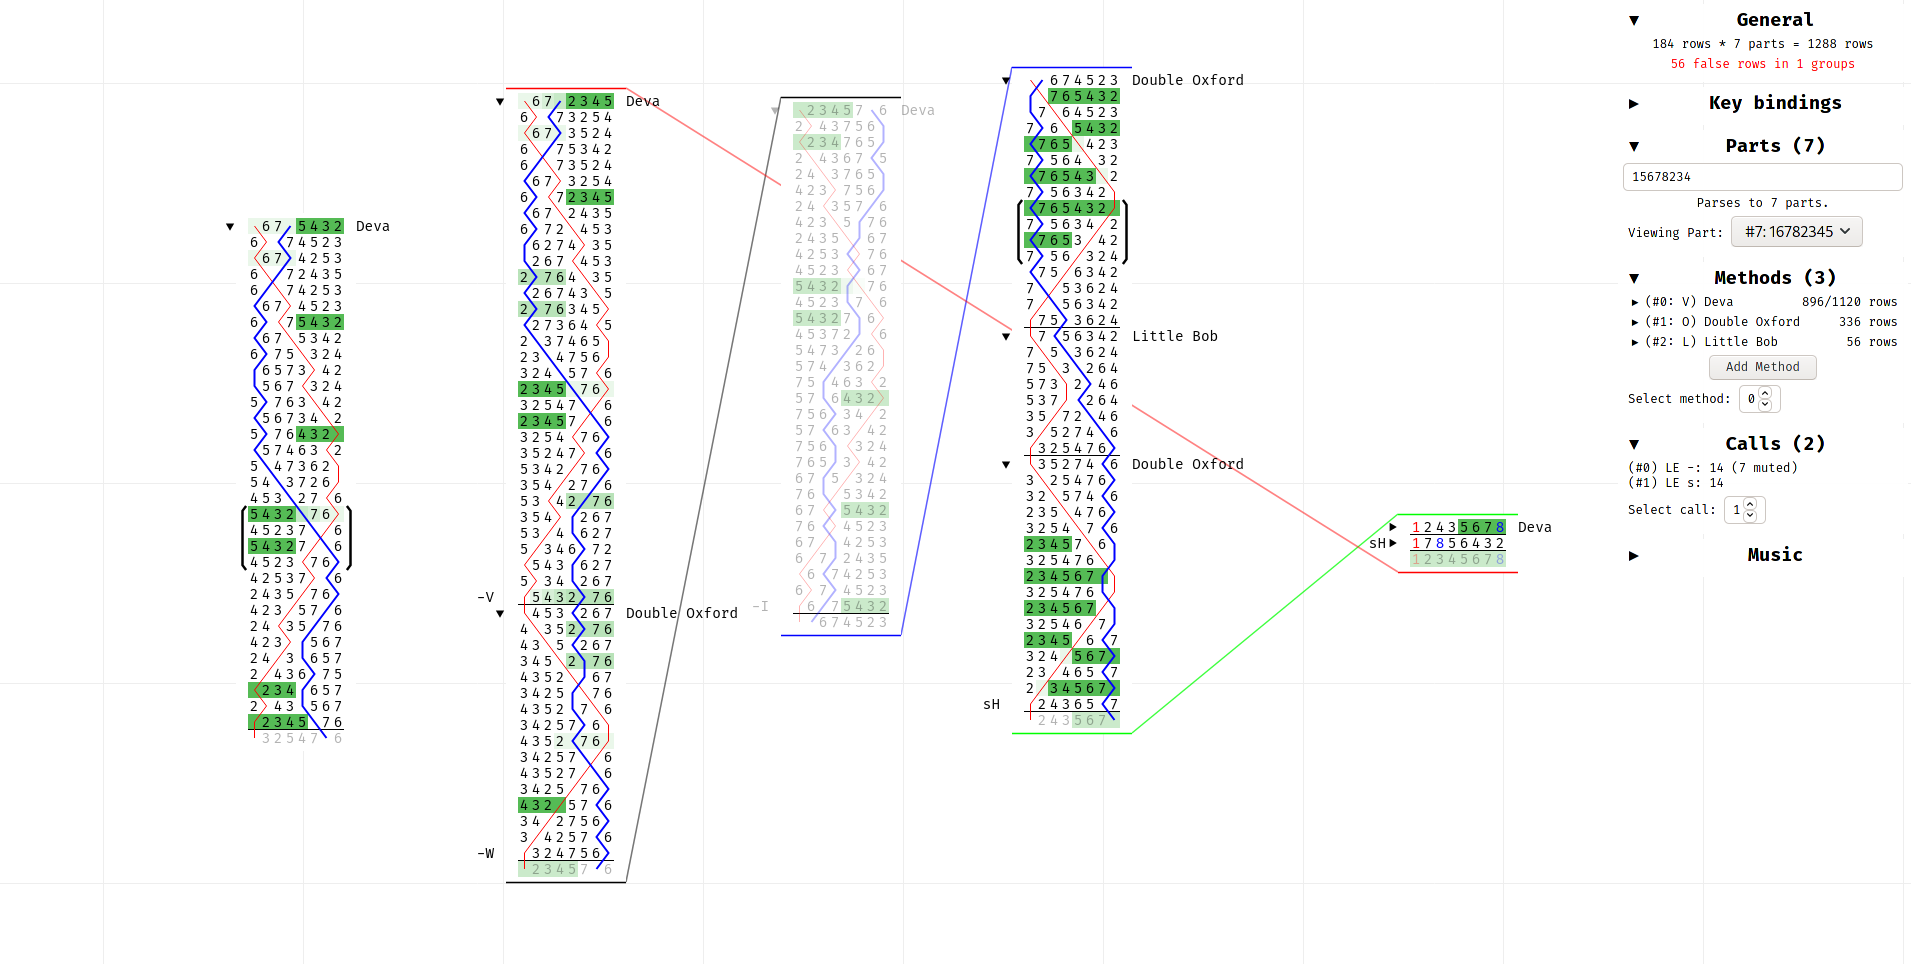
\includegraphics[width=\textwidth]{false-qp}
    \caption{Editing a Quarter Peal composition}\label{fig:cur-screenshot}
\end{figure}

\subsubsection{Static Web Application}

Jigsaw is built to be run as a single static web page (i.e.\ it is a fixed set of files that can be
served by a simple HTTP server).  Releasing applications as static websites has many advantages:

\begin{enumerate}
    \item There is no start-up time for a new user --- they open the page in any browser and the
        application starts immediately.
    \item HTML canvas rendering (while extremely inefficient compared to OpenGL or Vulkan) is easy,
        fast enough to feel instant and looks consistently good across all browsers and operating
        systems.

        The performance worries also turn out to be a non-issue; after implementing culling of
        off-screen rows, I have had no issues with rendering performance (at least on my new PC).
        There is also a lot of low hanging fruit for optimising the rendering, making this an
        entirely fixable issue.
    \item Having no dependence on a server both obviates the need for the user to make an account
        (which worsens the user experience) and also means that it can be deployed for free using
        GitHub pages or a similar service.
\end{enumerate}

Persistent storage is a challenge of static web applications, since websites can't directly access
the file system for security reasons.  Cookies are one possible option but they are sent over the
network with every request, making them completely unsuitable for storing large amounts of data.
Browsers do provide a persistent cache for network requests which can be arbitrarily read from and
written to, thus providing persistent storage.

\subsubsection{JavaScript and Rust/WebAssembly}

For the user interface, native web languages (JavaScript, HTML and CSS) are the obvious choice.  The
`back-end' of Jigsaw, however, has to do a lot of complex operations on data every time the user
changes the composition being displayed.  This must be done quickly enough that the user cannot
perceive the delay, and must be reliable.

JavaScript is very unsuitable for this kind of workload.  Firstly, it has no static analysis
whatsoever, making it unnecessarily difficult to write complex code correctly.  It also has no
control over memory layout and is absolutely reliant on a JIT (Just In Time) compiler to get good
performance.  Jigsaw's compute pipeline consists of several thousand lines of code, which is
unlikely to all be compiled by the JIT compiler.


Therefore, another language is required.  Jigsaw's back-end is written in Rust, a systems
programming language which emphasises performance and safety (the two things Jigsaw needs).  The
Rust code is compiled to WebAssembly so it can run natively in the browser.  Other languages could
work for this purpose (for example TypeScript, C/C++ or Go) but I chose Rust for the following
reasons:

\begin{enumerate}
    \item Rust gives you direct control over memory layout which provides excellent performance when
        manipulating complex data structures.  The performance of TypeScript, for instance, is by
        definition no better than that of JavaScript.
    \item The Rust compiler performs a large amount of strict compile-time correctness checks on
        your code, making it easy to implement complex algorithms in ways that you know is correct
        and fast.  C/C++ and Go cannot compete in this regard.
    \item Rust has first class support for WebAssembly.  Jigsaw was greatly aided by
        \verb|wasm_bindgen|, which generates binding code between native Rust and native JavaScript
        to let the two languages interface seamlessly.
    \item I am already proficient in Rust, so no time will be spent learning new languages for the
        project.
\end{enumerate}

\subsubsection{BellFrame}

\subsubsection{Code Architecture\ldots}



\pagebreak

\section{Overview of Change Ringing}

This project is to build a tool to help composers design complex sequences of ringing of church
bells.  Change ringing is a very niche and varied activity so this section will serve as a quick
introduction to the topic and overview of the aspects of change ringing which are most relevant to
this project.  A more complete overview can be found
on Wikipedia\footurl{https://en.wikipedia.org/wiki/Change_ringing}.

\br{}Change ringing (sometimes known as full-circle church bell ringing) originated in English
churches in around 1600, where churches began hanging sets of tuned bells on wheels in towers.
The installations range from 3 to 16 bells, with even numbers from 6 to 12 being almost ubiquitous.
These bells are typically quite heavy (bells over a ton are fairly common) and are spun
back and forth through 360 degrees like a pendulum.  All the bells are rung once in a sequence which
changes each time.  A piece of change ringing is a sequence of permutations, known as `changes'
(hence `change ringing').  Bells only move by at most one place between two adjacent rows.  On
paper, we write these permutations in order as rows of numbers and by convention, the bells
are numbered sequentially with `1' referring to the highest-pitched bell in the tower.  For
example:

\begin{verbatim}
12345678
21436587
21345678
12436587
12345678
\end{verbatim}

\subsection{Methods}
A performance of ringing will often contain thousands of individual rows.  Physical aids to memory
are not permitted during performances so the ringers must ring thousands of unique rows completely
from memory.  Memorising them all directly is clearly not feasible, so compositions are built up
from repeating patterns known as `methods'.

A method has a name (often with historical or geographical connections). In the method each bell
moves through a pre-determined path, moving back and forth within the sequence. Ringers learn this
path to help them remember where to ring in the sequence of rows.

\begin{wrapfigure}{r}{0.2\textwidth}
\centering
\begin{BVerbatim}
12345678
21436587
24163857
42618375
46213857
64128375
61482735
16847253
--------
16482735
61847253
68174523
86715432
87614523
78165432
71856342
17583624
--------
17856342
\end{BVerbatim}
\caption{Two leads concatenated}\label{fig:two-leads-lb8}
\end{wrapfigure}

A single instance of a method is called a `lead' and can be thought of as a super-permutation; it
takes a start row and produces a sequence of rows, ending with the row which the next lead should be
started (rows like this are not considered part of the super-permutation).

For example, the following are all leads of the same method\footnote{This particular method is known
as `Little Bob Major'.} (we write the `leftover' row under a dashed line because it belongs to the
lead \emph{after} the others):

\begin{multicols}{3}

\centering
\begin{BVerbatim}
12345678
21436587
24163857
42618375
46213857
64128375
61482735
16847253
--------
16482735
\end{BVerbatim}

\centering
\begin{BVerbatim}
16482735
61847253
68174523
86715432
87614523
78165432
71856342
17583624
--------
17856342
\end{BVerbatim}

\centering
\begin{BVerbatim}
12486753
21847635
28174365
82713456
87214365
78123456
71832546
17385264
--------
17832546
\end{BVerbatim}

\end{multicols}

Note that a single lead of this method preserves the location of the bell at the start of the
row.  This is an extremely common feature of methods because it allows ringers to orient
themselves around this `fixed' bell and therefore helps prevent mistakes.

One observation we can make here is that the second column begins with the leftover row of the
first.  Therefore, we could concatenate the two leads together to form a longer piece (as in
Figure~\ref{fig:two-leads-lb8}). Note how the dashed lines split consecutive leads.

\subsection{Compositions}

A `composition' is a sequence of rows of some length which satisfies the adjacency property and
starts and finishes with the row containing bells in descending order (\row{123456\ldots}, known as
`rounds').  Thus, the above diagram shows a valid composition.

The task of a composer is to create compositions which have some set of desirable features (which is
likely to depend heavily on the circumstances of each performance).  In order to understand the
rationale behind this project and gauge its success, we must first understand some of the most
important features or constraints of compositions.

\subsection{Features of Compositions}

\subsubsection{Truth/Falseness}

A composition is called \emph{true} if every row is unique, and is called \emph{false} otherwise.
This is \emph{the} most important property that a composition must have, since any performance of a
false composition is considered invalid and therefore a waste of the ringers' time.  When we write
out compositions we usually write out rounds twice, but when considering falseness it is only
counted once (thus, rounds in the middle of a composition is still false).

\subsubsection{Length}

The `length' of a composition is the number of rows which it contains.  Like falseness, external
rounds is only considered once.  90\% of performances have one of two length ranges:

\begin{enumerate}
    \item A \textbf{Peal} consists of at least 5000 rows (about 3 hours' of ringing).
        The number 5000 is chosen because historically the pinnacle of ringing challenge was to ring
        every permutation of 7 bells, which results in $7! = 5040$ rows.  This was recently rounded
        down to 5000 for all numbers of bells, but the majority of people prefer the completeness of
        5040 rows for peals of 5, 6 or 7 bells (where every possible row is rung the same number of
        times).
    \item A \textbf{Quarter Peal} consists of at least 1250 rows (a quarter of a peal's length, and
        about 45 minutes of ringing).  Due to the reduced completion time, these are much more
        common than peals.  Half peals ($\ge 2500$ rows) and double-length peals ($\ge 10,000$ rows)
        are both recognised lengths but performances of them are very rare.
\end{enumerate}

Also, every row above the lower bound is extra ringing time for little gain in performance merit,
and therefore composers try to make compositions which are fairly tight to these lower bounds.
Indeed, lengths within the ranges $1250 \le l < 1300$ or $5000 \le l < 5100$ are almost ubiquitous.

\subsubsection{Music}

If we are composing for $\ge 8$ bells, then our composition will not contain every possible row and
we therefore have the opportunity to decide which rows get included and which don't.  Of these, some
may be more favourable than others.

Currently, people like rows which start or finish with at least 4 consecutive bells.  The exact bells
are unimportant and the longer the run the better.  For example \row{34567812} starts with a
descending run of 6 bells, and is therefore preferable to \row{57864321} which ends with an
ascending run of 4 bells.  Both of these are preferable to \row{18346527} which has no runs
whatsoever.

\subsubsection{Complexity}

Complexity does not have a nice mathematical definition and therefore this project will make no
attempt to automate it.  However, it is still an important concept which roughly corresponds to how
repetitive and predictable is your composition.

In general, we want to make these things as simple as possible because that will open your
composition to the most potential bands.  However, sometimes \emph{the point} of a composition is to
be a challenge, in which case complexity is fair game.

\subsubsection{Summary}

In general, length and falseness are hard constraints which composers have little choice over and
must work around.  Most of the time, the composer fixes some target level of complexity and tries
to get as much music or interest as possible within that constraint.  Also, many composers make
compositions that they intend to conduct themselves, allowing for a higher level of complexity
because they already have an intimate knowledge of the composition when learning it.



\pagebreak

\section{Design}

The overall design of Jigsaw is an infinitely scrollable canvas which contains any number of
fragments in any location.  It is also designed to be used on a desktop with a 3-button mouse and
keyboard, and for maximal efficiency all common operations are triggered by keys on the left side of
the keyboard.  For consistency, all operations are applied at the location of the mouse cursor.

Overlaid on this canvas is a sidebar containing information which can't be represented using the
canvas interface.  This contains a lot of dense information, so all sections can be folded to only
show what's relevant.

// List of keyboard shortcuts/operations

Fragments can be created or extended with \verb|a| (a single lead) or \verb|A| (a full course).

\begin{figure}
    \centering
    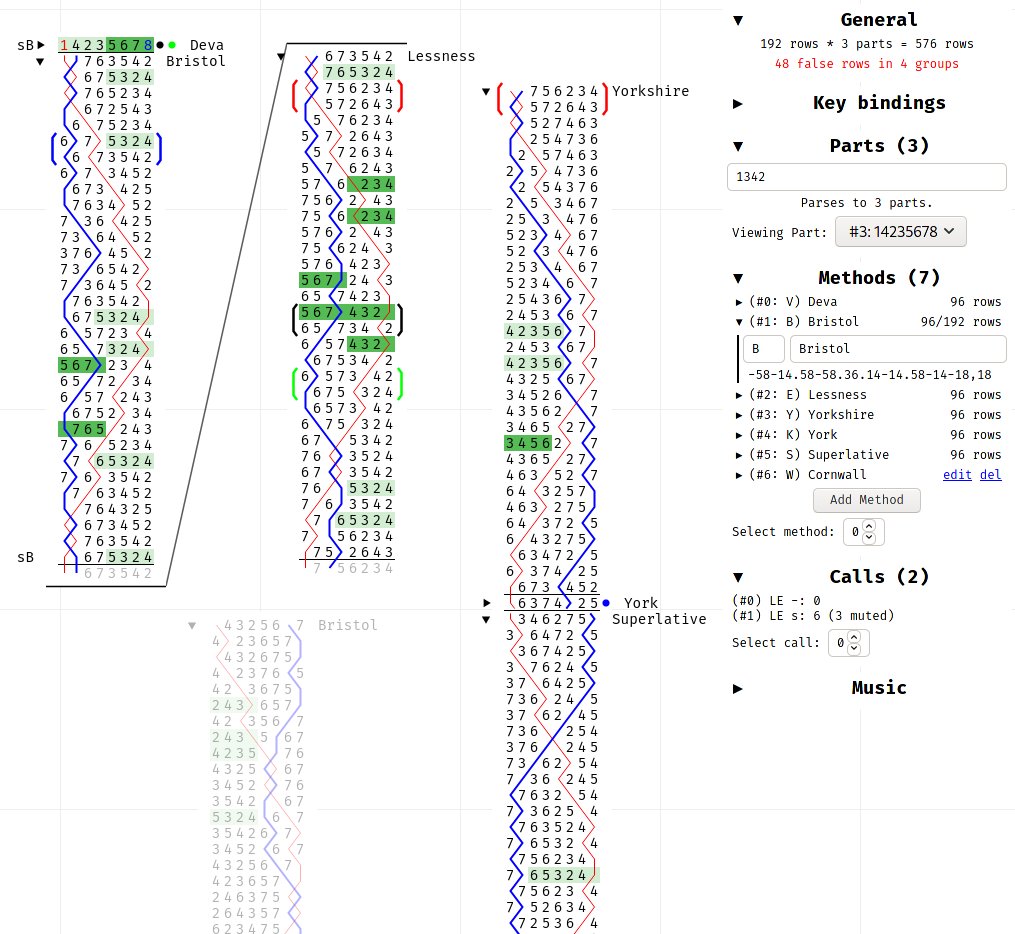
\includegraphics[width=0.8\textwidth]{current-screenshot-w-mute}
    \caption{Screenshot of Jigsaw, showing the folding UI and canvas display}\label{fig:cur-screenshot}
\end{figure}

\subsection{Music Highlighting}

When music appears in a composition, the bells causing the music are highlighted green, giving an
an obvious visual indication of where the music is.

Additionally, non-musical rows can generate music in other parts of the composition, and in this
case the music is `onion-skinned' --- the more parts contain music, the darker the colour.  In
Figure~\ref{fig:multi-part-music}, for example, \row{4328} in the \nth{1}{st} lead is highlighted quite
densely because it generates \row{5432}, \row{6543}, etc.\ in other parts.  However, \row{8761} in
the \nth{4}{th} lead is highlighted very lightly because it only creates \row{4321} in the \nth{2}{nd}
lead.

\begin{figure}
    \centering
    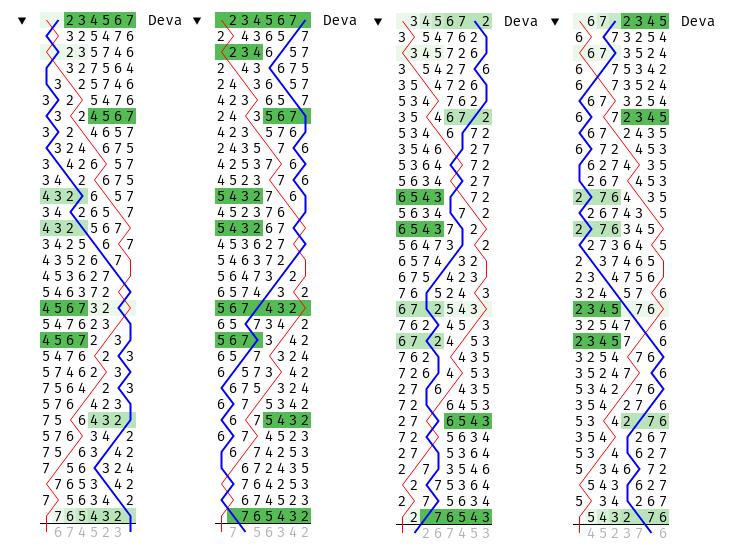
\includegraphics[width=0.6\textwidth]{multi-part-music-clean}
    \caption{The same lead in four different parts (rotating 2--8)}\label{fig:multi-part-music}
\end{figure}

\subsection{Falseness Display}

Falseness is visually communicated by marking groups of identical rows with the same coloured
brackets (see Figure~\ref{fig:falseness}).  As far as I know, this is the most efficient way of
visually communicating exact falseness.  The main drawbacks of this approach is that the number of
different groups can get very large causing Jigsaw to run out of easily differentiable colours.
Additionally, it is very reliant on colours which will likely be problematic for colour-blind
people.  A fix for this would be to add a switch to number the groups rather than just relying on
colour.

\begin{figure}
    \centering
    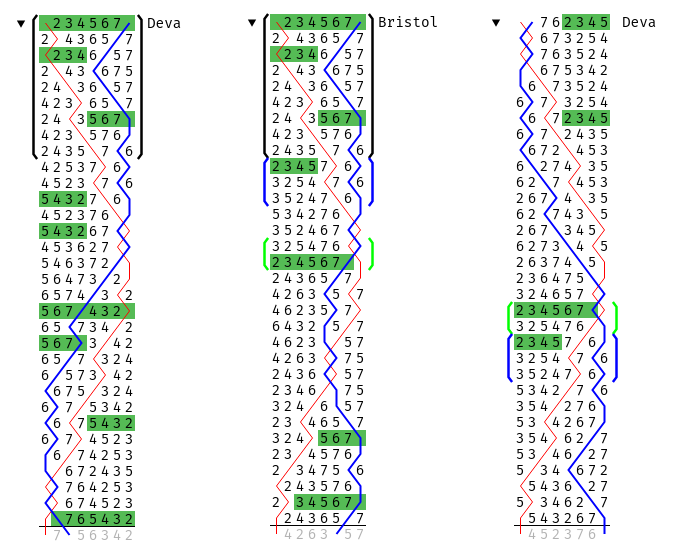
\includegraphics[width=0.5\textwidth]{falseness-clean}
    \caption{Leads which are false in 3 different ways}\label{fig:falseness}
\end{figure}

\subsection{Lead Folding}

To prevent the user from having to look at thousands of rows at the same time, Jigsaw allows leads
to be folded into a single row.  Jigsaw then converts falseness groups into dots next to the row
number (see Figure~\ref{fig:lead-folding}), and switches between lines and numbers for displaying
bells when necessary.

\begin{figure}
    \centering
    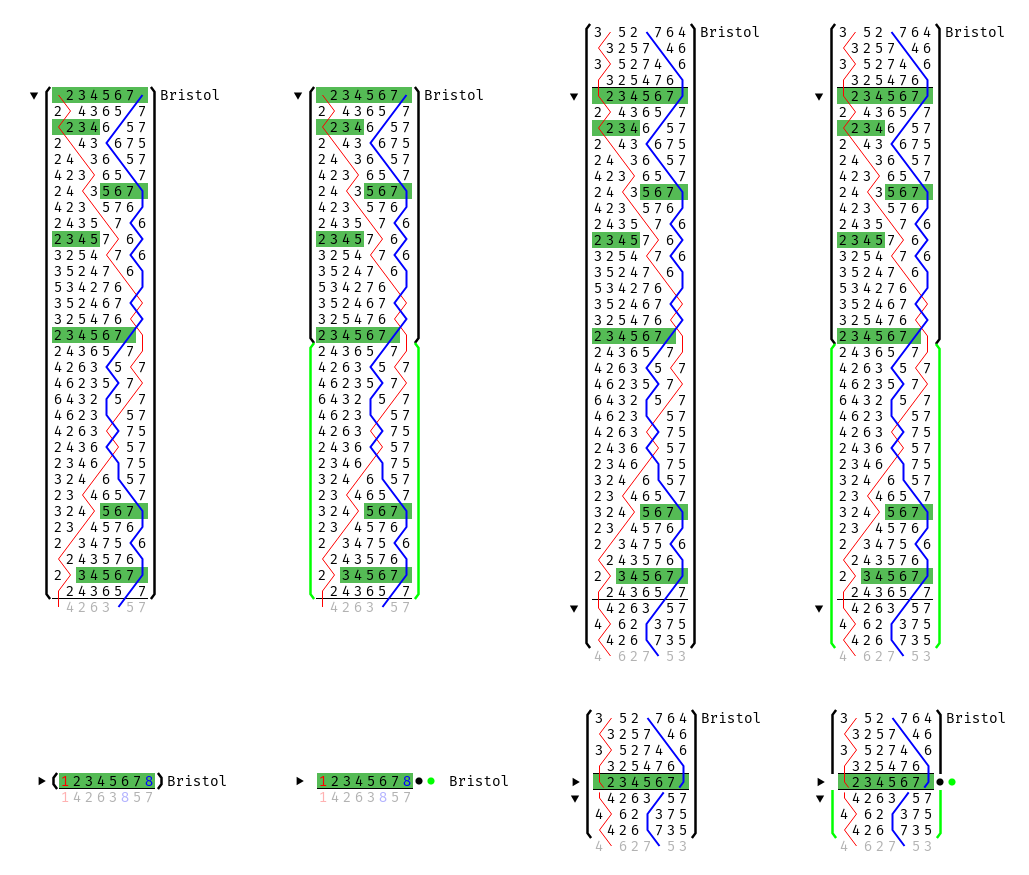
\includegraphics[width=0.78\textwidth]{folding-full}
    \caption{Unfolded (top) and folded (bottom) versions of the same lead.  Note the handling of
    falseness ranges and line segments.}\label{fig:lead-folding}
\end{figure}

\subsection{Linking Fragments}

Two fragments can be linked together if the leftover row of one is equal to the first row of the
other.  To represent this visually, Jigsaw draws a coloured line between the two (see
Figure~\ref{fig:linking}).  If multiple different sets of fragments link, then each group is
coloured separately (see Figure~\ref{fig:linking-insane}).

Hovering a line and pressing \verb|c| (for `connect') will join those fragments into one.  Note how
this operation doesn't change the rows contained in the composition.

\begin{figure}
    \centering
    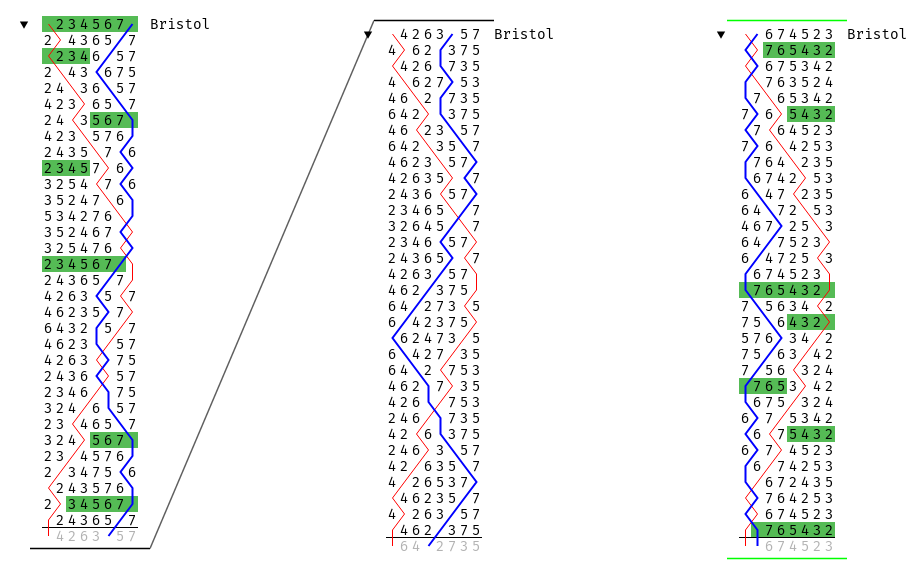
\includegraphics[width=0.8\textwidth]{linking-2}
    \caption{Two fragments which link together, and one that links to itself.}\label{fig:linking}
\end{figure}

\begin{figure}[h!]
    \centering
    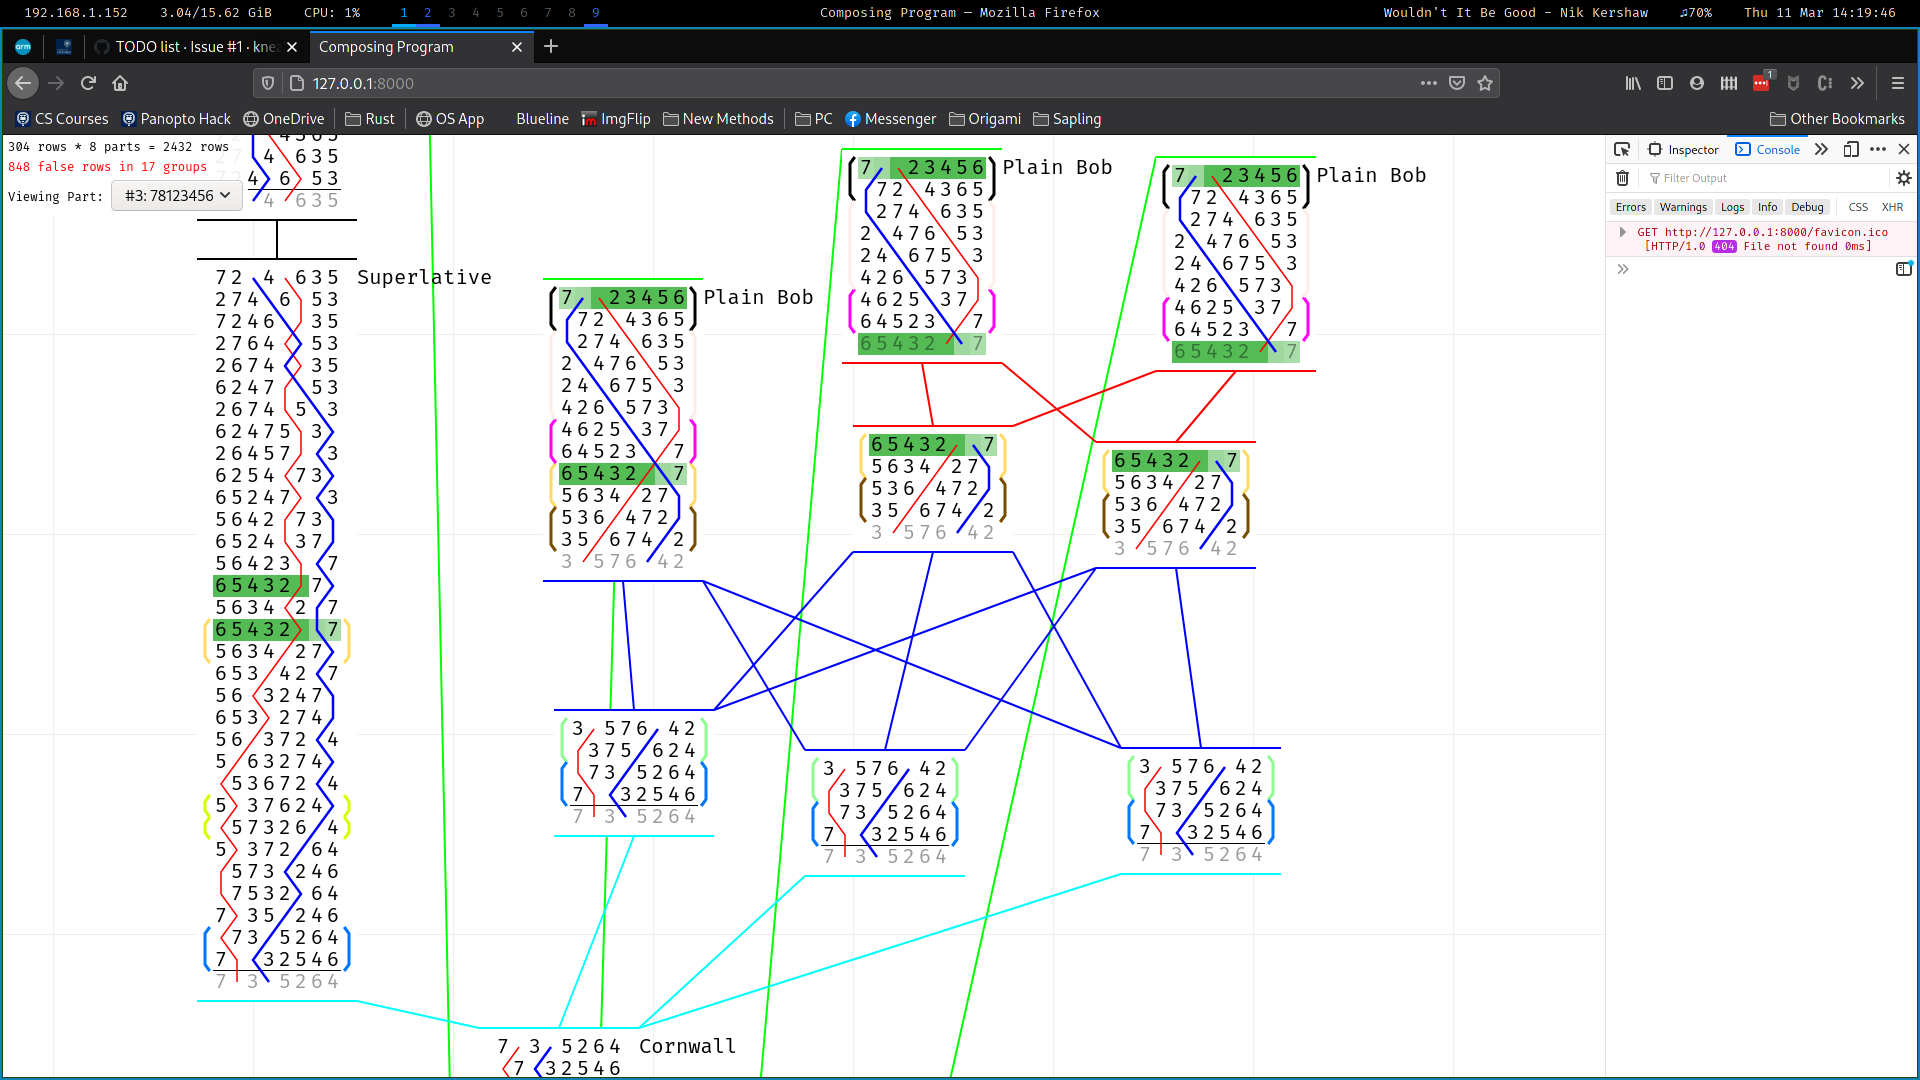
\includegraphics[width=\textwidth]{linking-insane}
    \caption{A lot of fragment links on one screen.}\label{fig:linking-insane}
\end{figure}



\pagebreak

\section{Implementation}

The code for Jigsaw is split into 3 main parts: two Rust libraries which together form a `server'
and `client' in the form of a web GUI.\@  The Rust code is compiled to WebAssembly, and exports an
API which allows the JavaScript client to make changes to the internal `model' and then request a
JSON serialisation of the information to display to the user.

This architecture plays to the strengths of both languages --- Rust provides fast and reliable data
manipulation whilst JavaScript, HTML and CSS provide a user-friendly cross-platform GUI.\@  The
binding and serialisation code is automatically generated at compile time using
\emph{wasm-bindgen}\footurl{https://github.com/rustwasm/wasm-bindgen} and
\emph{serde}\footurl{https://github.com/serde-rs/serde} to prevent human error.

\subsection{BellFrame}

Roughly half of the Rust code in the project is a cross-platform utility library for core datatypes
which are not specific to Jigsaw.  This provides safe and performant Rust datatypes for common
constructs related to change ringing (\verb|Row|, \verb|Bell|, \verb|Method|, \verb|Call|, etc.).
Its development and API design was motivated by Jigsaw but once its API is stable it will be
published to Rust's central package repository for general use.

The stable part of the API has good documentation and is well tested, and all datatypes only provide
public functions which preserve internal invariants and therefore obviate the need for unnecessary
checks.  It also provides `unsafe' versions of functions which remove runtime checks but in rely on
their caller to uphold the invariants.  Therefore, no undefined behaviour is possible if the user
only writes `safe' code.

Despite have no stable API, I have already built other projects on it.  In its own right, this
library is a valuable product of this project.

\subsubsection{Aside: Rows vs Permutations}

When writing BellFrame, I initially thought that the concept of rows and permutations were different
enough to warrant separate data types.  My thinking was that a \verb|Row| is a sequence of
\verb|Bell|s (plus some additional invariants), and a permutation can be thought of as a function of
type \verb|[a] -> [a]| which can permute sequences of any type.  Mathematically this feels like an
elegant separation, but using the library in earnest made me realise that the \verb|Perm| doesn't
pull its weight given its large overlap with the \verb|Row| type.  I would almost always use
\verb|Perm| only as an intermediate step to use one \verb|Row| to permute another.  Therefore, a few
months into the project the operations of the \verb|Perm| structure was merged into \verb|Row|.

\subsection{Model-View-Presenter}

The code in the jigsaw library differentiates between the unique specification of a composition
(the \verb|Spec| type) and the information required to display it to the user (the
\verb|DerivedState| type).  The \verb|DerivedState| contains additional data like the music
locations, falseness and other annotations which are completely specified by the current
\verb|Spec| but necessary for displaying a composition.  Every change to the \verb|Spec| also causes
the \verb|DerivedState| to be updated before the changes can be displayed to the user.

Figure~\ref{fig:model-view-presenter} shows how Jigsaw's code maps to Model-View-Presenter.
Additionally, the Model-View-Presenter means that every edit passes completely through the model,
resulting in a data flow shown in Figure~\ref{fig:app-data-flow}.

\iffalse
\subsection{Data Flow}

These invariants enforce a very specific data flow whenever the user changes the composition
(summarised in Figure~\ref{fig:app-data-flow}).  The user's input events are all captured by
JavaScript, which calls a corresponding function in \verb|Comp|'s API.\@ The \verb|Comp| singleton
then clones the current \verb|Spec|, performs the required modifications and then pushes it onto the
history stack.  Next, \verb|Comp| rebuilds its copy of \verb|DerivedState| to reflect the changes in
the \verb|Spec| (thus upholding the invariants).  At this point, the WebAssembly function returns
control to JavaScript which immediately calls \verb|Comp::ser_derived_state| which returns a JSON
string with which to overwrite the \verb|derived_state| variable.
\fi

\begin{figure}
    \centering
    \begin{BVerbatim}
   +------------------------+
   |    View (JavaScript)   |
   +------------------------+
           |         ^
Comp's API |         | Comp::ser_derived_state
           V         |
   +------------------------+
   |        Presenter       |
   |  (Comp, DerivedState)  |
   +------------------------+
           |         ^
     Edits |         | DerivedState::from_spec
           V         |
   +------------------------+
   |       Model (Spec)     |
   +------------------------+
    \end{BVerbatim}
    \caption{Jigsaw's implementation of model-view-presenter}\label{fig:model-view-presenter}
\end{figure}

\begin{figure}
    \centering
    \begin{BVerbatim}
        JS          |        Rust
--------------------+--------------------
     User input     |
         |          |
         V      API Call
       Event -------------> Comp API
         |          |          |
         |          |          V
         |          |      Clone Spec
         | undo/    |          |
         | redo     |          V
         |          |    Modify new Spec
         |          |          |
         |          |          V
         \-------------> Update History
             API Call          |
                    |          V
         /------------ Rebuild DerivedState
         |   return |
         |          |
 sync_derived_state |
         \-------------> ser_derived_state
             API Call          |
                    |       (serde)
                    |          V
   JSON String <--------- JSON String
        |        return
  (deserialise)     |
        V           |
  derived_state     |
        |           |
        V           |
     repaint        |
    \end{BVerbatim}
    \caption{The data flow of user's changes}\label{fig:app-data-flow}
\end{figure}

\subsection{Specification vs Derived State}

The code in the jigsaw library differentiates between the unique specification of a composition
(the \verb|Spec| type) and the information required to display it to the user (the
\verb|DerivedState| type).  The \verb|DerivedState| contains additional data like the music
locations, falseness and other annotations.  That is completely specified by the contents of the
current \verb|Spec|, so every change to the \verb|Spec| must also cause the \verb|DerivedState| to
be updated before the changes can be displayed to the user.

In terms of Model-View-Presenter, the \verb|Spec| type is the Model whereas the \verb|DerivedState|
is the data sent from the Presenter to the View.

\subsection{Undo History}

Jigsaw uses the `immutable data structure' method of storing undo history, where the history is a
sequence of fully defined states (as opposed to an event system where the history is a sequence of
modifications).  Therefore, the undo history is simply a list of \verb|Spec| types along with an
index referring to the `current' \verb|Spec| being displayed on the screen.

In order to prevent unnecessary duplication of data, the internal data of the \verb|Spec| type is
always stored behind reference counted pointers.  Therefore, cloning a \verb|Spec| adds one to the
reference count rather than cloning the backing data.  If we need to modify a part of the data, then
we have to clone it using \verb|Rc::make_mut| provided by the standard library.  Rust checks this
at compile-time and will reject code which tries to modify shared data without first cloning it.

This approach works excellently, and allows Jigsaw to fully update the display without adding steps
to the undo history.  This gives the user instant feedback when transposing fragments.

\subsubsection{Aside: Passing Data Between Rust and JavaScript}

Even with \emph{wasm-bindgen} providing binding code, the types that can be sent over the language
interface is limited to flat structures with no references.  This is unfortunate, since the
\verb|DerivedState| has 4 layers of references (\verb|DerivedState| $\to$ \verb|DerivedFrag| $\to$
\verb|DisplayRow| $\to$ \verb|Row| $\to$ \verb|Bell|), all of which is required to render each
frame.  Therefore, it isn't possible to simply return the \verb|DerivedState| from Rust into
JavaScript, and another strategy is required.

Initially, I didn't want JavaScript and Rust to hold their own copies of \verb|DerivedState|,
because then there would be two potentially divergent sources of the truth (causing bugs which would
be extremely hard to fix).  Additionally, I wanted to limit the complexity handled by the JavaScript
code (due to its inferior performance and maintainability) so it felt natural for Rust to handle all
the state and then expose a simple API to JavaScript to read the data.

The original API was a flat set of getter functions, looking like Figure~\ref{fig:initial-api}.
This worked fine for a while but as the complexity of \verb|DerivedState| grew, the number of
exported functions exploded and refactoring the API became unnecessarily challenging.  Also, every
WebAssembly function call takes a non-trivial amount of time and this flat API encourages huge
numbers of calls each frame which started causing performance issues.  It's also worth noting that
the \verb|DerivedState| only changes when the user changes the composition, but is needed every time
the UI is painted.

\begin{figure}
    \begin{verbatim}
/// Get the number of fragments
fn get_num_frags() -> usize { ... }

/// Get the number of rows in the fragment at a given index
fn get_frag_length(frag_index: usize) -> usize { ... }

/// Get the bell at a given location
fn get_row(
    frag_index: usize,
    row_index: usize,
    bell_index: usize
) -> Bell { ... }
    \end{verbatim}
    \caption{Initial getter API design}\label{fig:initial-api}
\end{figure}

Eventually, I settled on the strategy that Jigsaw currently uses:  to pass the entire
\verb|DerivedState| structure as a JSON string
after each edit.  JavaScript then parses and caches the resulting object which it reads from when
drawing each frame.  This turned out to work really well --- almost no WebAssembly calls are made
during each frame, the `getter' API is reduced to a single function and long-term divergence is
still impossible because JavaScript completely overwrites its copy of the \verb|DerivedState| each
time the composition updates.

The serialisation code is generated at compile-time using \emph{serde}
(\url{https://github.com/serde-rs/serde}), removing the possibility for human error.  Therefore, the
data in JavaScript and Rust will always have the same structure, making the whole code base much
easier to read and refactor.



\pagebreak

\section{Conclusion}

This project has two major products: the application itself (named Jigsaw) and the reusable utility
library on which Jigsaw is built (named BellFrame).

As it stands right now, I think that BellFrame is a bigger contribution to composing (despite
technically being a bi-product) since it is very usable and has some battle-testing.  Jigsaw, on
the other hand, is a very promising prototype but is not feature complete or stable enough to be
used in production.  Fixing both these issues is simply a matter of development time and testing, 
and I will continue working on Jigsaw even after this project is handed in.  Given the limited
time-frame of this project, I chose to spend it on exploring unexplored ideas rather than striving
for perfect stability.

\subsection{Jigsaw}

I think that Jigsaw is a successful prototype and I will likely continue building it into a
feature-complete application.  I demonstrated it to several other composers who all thought it
looked very promising.  It has a number of small rough edges which would make the current iteration
difficult to use in production, but do not detract from its value as a prototype.

In order to decide on the success of the project, I will rank it against the design goals set out in
Section~\ref{sec:design-goals}.

\subsubsection{Ease of Use \& Visual}

Firstly, building Jigsaw as a single static page means it requires no installation to use.  The
design of an infinite canvas plus a folding sidebar feels very natural and intuitive to use.

A large amount of effort went into making sure that GUI is visually crisp and responsive.  This
goes as far as rounding all coordinates to the nearest pixel to prevent fuzzy boundaries
(screenshot?), as well as doing the same for line rendering --- see
Section~\ref{sec:line-rendering}.  This attention to detail makes the experience of using Jigsaw
feel very smooth and polished.

All actions are currently bound to keyboard shortcuts which means that editing compositions quickly
becomes muscle memory for experienced users, but feels unintuitive to beginners since at any point
in time there's no indicator of what actions are available.  If I had more time, I would add a
contextual right-click menu to fix this problem (it could even show the key bindings to help
beginners learn them).

\subsubsection{Completeness}

Jigsaw's internal representation is complete, but the current user interface is not.  In other
words, Jigsaw is internally able to represent a strict superset of compositions which are considered
change ringing, but the prototype GUI means that the user is unable to express some very obscure
states which are technically considered change ringing.  For perhaps 99\% of use cases, Jigsaw's
user interface is complete enough that most users would not notice.

\subsubsection{Incremental}

Jigsaw is completely built around being incremental.  It also does its best to preserve `continuity'
of operations --- that is, a small operation should cause a small change to the composition's rows.
Some operations like splitting and joining fragments only change the structure of the composition,
and not the output rows.

\subsubsection{Instant}

Due to the internal architecture, the composition is always fully annotated.  Whenever the user
causes an update, the entire state of the display is recalculated then cached for repainting.
Therefore, it simply isn't possible for any part of the changes to lag behind because the full UI
state is simultaneously recalculated after every change.

This does, however, mean that Jigsaw is extremely dependent on the efficiency of this update
pipeline.  Luckily, Rust and WebAssembly seem to be working extremely well here since the pipeline
is fast enough to reliably feel instant, even for extremely large compositions.  I haven't done any
specific optimisations, but I have also been mindful of high-level performance when writing the code
--- the algorithms are all $O(n \log n)$ in the number of bells in the composition, although the
link detection is $O(n^2)$ in the number of fragments.

Whilst stress testing Jigsaw, I discovered that this delay becomes noticeable at around 35,000
$\times$ 8 = 280,000 bells (see Figure~\ref{fig:stress-test}).  Since at least 99.9\% of
compositions have at most 10,000 rows each of 16 bells (making 160,000 bells total) I think that the
performance is perfectly adequate.

The longest piece of ringing ever rung contains 72,000 $\times$ 6 = 432,000 bells, which would cause
the current implementation some consternation.  In reality, the composition for this was split into
many separate pieces to ease memorability so I doubt anyone would want to reason about the
composition in full.  However, I would like Jigsaw to eventually support huge compositions, and
there is plenty of low hanging fruit left to optimise --- for example, the pipeline does no caching
or re-use of memory allocations so the code generates huge numbers of needless allocations during
each pipeline run.

Lastly, BellFrame contains the \verb|SimdRow| type which uses SIMD instructions
(specifically \verb|pshufb|) to perform row permutations in a single clock cycle, which usually
increases performance by at least an order of magnitude.  However, SIMD support in WebAssembly is
not mainstream yet so Jigsaw can't take advantage of this.

\begin{figure}
    \centering
    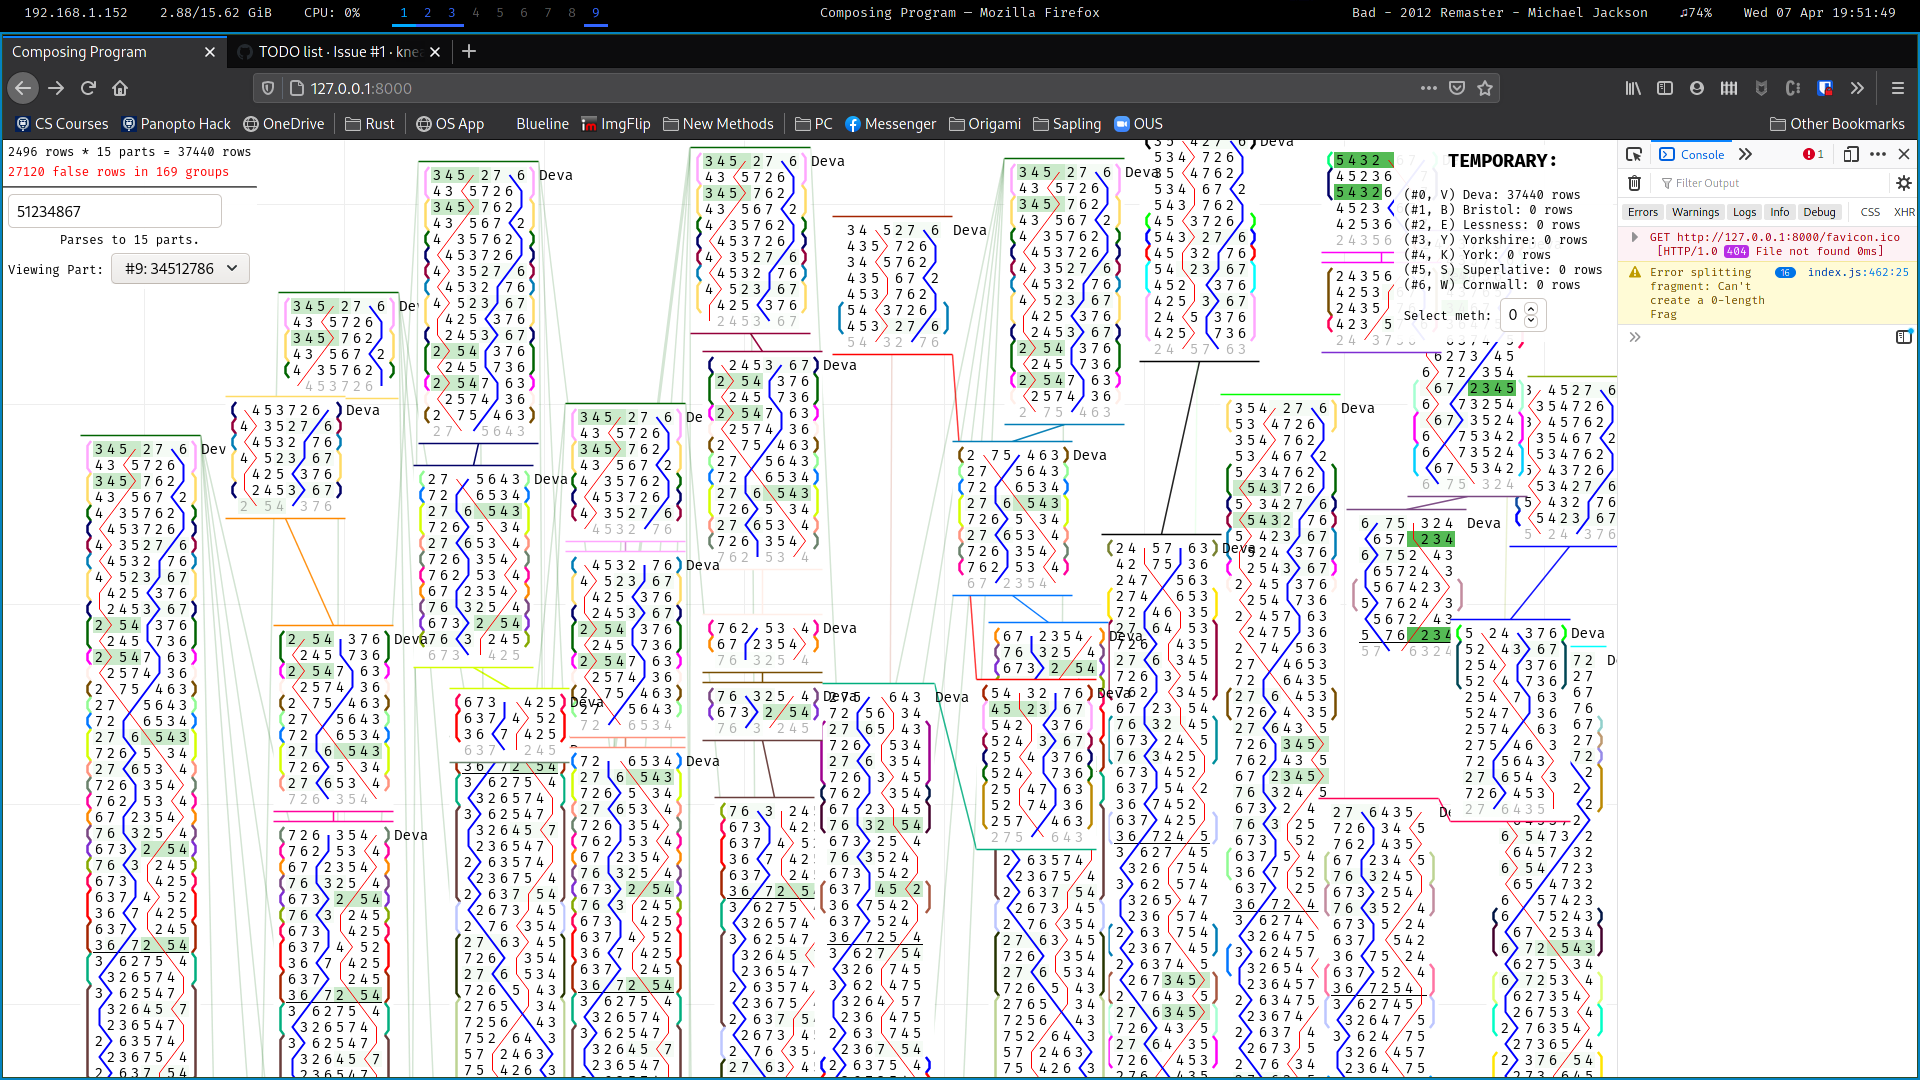
\includegraphics[width=\textwidth]{stress-test}
    \caption{Stress testing Jigsaw (the GUI has since changed, but the pipeline has
    not).}\label{fig:stress-test}
\end{figure}



\pagebreak

\section{Glossary of Change Ringing Terms}

\paragraph{Stage:} The number of bells which the composition uses.  This is not necessarily the
number of bells used to ring a given composition, but for the purposes of this project the
distinction is not relevant.

\paragraph{Row:} A sequence of bells which forms a permutation.  Rows are the fundamental building
blocks of compositions.  The words `change' and `row' are often used interchangeably (hence the name
`Change Ringing'), but to avoid confusion I will always use `row' in this report.

\paragraph{Composition:} An ordered sequence of rows which tell ringers in which order the bells
should be rung.

\paragraph{Truth:} For the purposes of this project, a composition is \emph{`true'} if all the rows
are unique, otherwise it is \emph{`false'}.  This is the single most important property of a
composition, since any performance of a `false' composition is considered invalid.

\paragraph{Method:} A short, usually symmetrical, pattern that is repeated throughout a composition
with small and well-defined modifications (known as `calls').  This is the key to how human ringers
can ring over 5000 rows worth of composition without any memory aid --- in reality, they memorise
the method(s) and one `conductor' memorises the pattern of calls and calls them in the right places
for the other ringers to take effect.  It is usually the job of the composer to make sure that the
call sequence is predictable and easy to memorise.

\paragraph{Lead:} A single instance of the repeating pattern of a method.

\end{document}
